\section{Comparaison avec la photo aux couleurs
inversées}\label{comparaison-avec-la-photo-aux-couleurs-inversuxe9es}

\begin{figure}[htbp]
\centering
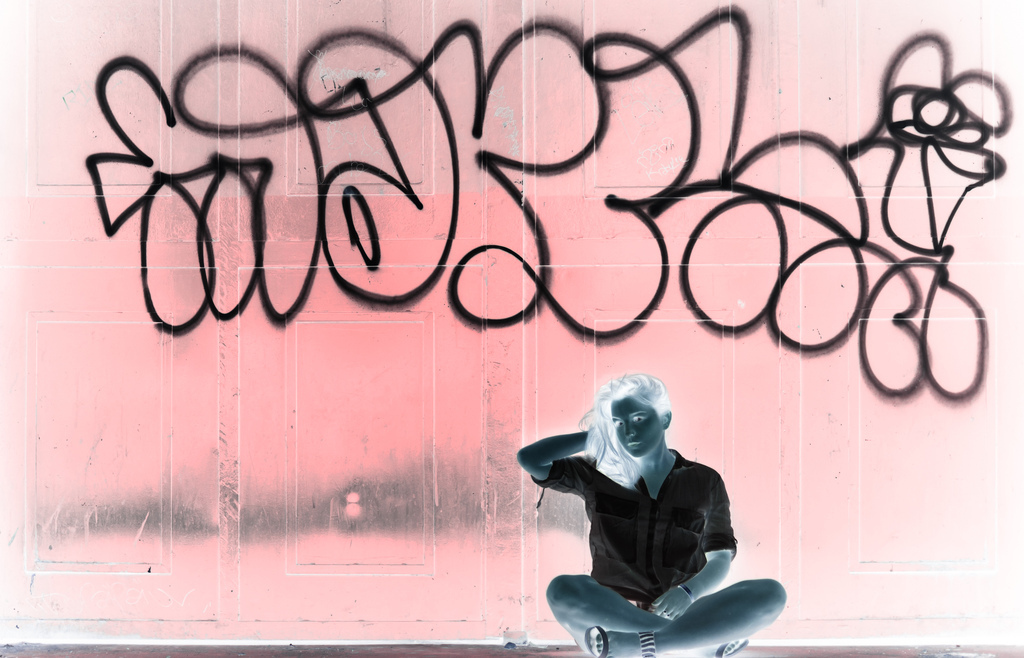
\includegraphics{../../photos/inverse.jpg}
\caption{Photo couleurs inversées}
\end{figure}

\begin{table}[htbp]
\centering
\begin{tabular}{llr}
\bfseries Formes &
\bfseries Bhattacharyya (\%)%
\DTLforeach*[\DTLiseq{\fichier}{photos/inverse.jpg}]{valeurs}{%
\fichier=Fichier, \formes=Formes,\bhatta=Bhattacharyya, \hue=Hue, \saturation=Saturation, \value=Value}{%
\\
\formes & \bhatta}
\end{tabular}
\end{table}

Les résultats de la comparaison de la photo originale avec la photo inversée
nous montre une différence de formes nulle via la comparaison des photos en
Sobel et une différence de $49.49 \%$ en distance de Bhattacharyya. \\
Cela s'explique par le fait que l'inversion des couleurs ne change pas les
formes de la photo.
